\documentclass[NET,english,beameralt]{tumbeamer}

% If you load additional packages, do so in packages.sty as figures are build
% as standalone documents and you may want to have effect on them, too.

% Folder structure:
% .
% ├── beamermods.sty                  % depricated an will be removed soon
% ├── compile                         % remotely compile slides
% ├── figures                         % all figures go here
% │   └── schichtenmodelle_osi.tikz   % each .tikz or .tex is a target
% ├── include                         % create your document here
% │   ├── example.tex                 % example document
% │   └── slides.tex                  % make document wide changes here
% ├── lit.bib                         % literature
% ├── Makefile
% ├── moeptikz.sty                    % fancy networking symbols
% ├── packages.sty                    % load additional packages there
% ├── pics                            % binary pcitures go here
% ├── slides.tex                      % main document (may be more than one)
% ├── tumbeamer.cls
% ├── tumcolor.sty                    % TUM color definitions
% ├── tumcontact.sty                  % TUM headers and footers
% ├── tumlang.sty                     % TUM names and language settings
% └── tumlogo.sty                     % TUM logos

% Configure author, title, etc. here:
\usepackage[utf8]{inputenc}
\usepackage{packages}
\usepackage{beamermods}

% For beamer mode (default):
\author[S. G\"unther]{Stephan Günther}
\title[Networking]{Something with Networking}

% Uncomment to add advisors for presentation in Oberseminar
%\advisor{Herrmann B. Wolfgang}

% Uncomment to add type for presentation in Oberseminar
% Usage: \thesistype{intermediate | final}{bachelor | master | idp | gr}
%\thesistype{intermediate}{gr}

% Uncomment to configure date in dd-mm-yyyy format
%\newdate{date}{25}{05}{2017}
%\date{\displaydate{date}}

% Uncomment to add a venue to the title slide
%\venue{International Conference on Conferencing 2018 \\ Garching b. München, Germany}

% For lecture mode (use package option 'lecture'):
%\lecture[GRNVS]{Grundlagen Rechnernetze und Verteilte Systeme}
%\module{IN0010}
%\semester{SoSe\,2016}
%\assistants{Johannes Naab, Stephan Günther, Maurice Leclaire}


\usepackage{pgfpages}
\usepackage{ifthen}
% ============================================================================
% jobname solution
% ============================================================================
\newif\ifsolution%
\ifthenelse{\equal{\detokenize{notes}}{\jobname}}{%
\setbeameroption{show notes on second screen=bottom}
\setbeamercolor{note page}{bg=white, fg=black}
\setbeamercolor{note title}{bg=white!95!black, fg=black}
}{
}

% TeXLive 2018 compatibility: https://tex.stackexchange.com/questions/426088/texlive-pretest-2018-beamer-and-subfig-collide
\makeatletter
\let\@@magyar@captionfix\relax
\makeatother


\begin{document}

% If you are preparing a talk but do not like the default font sizes, you may
% want to try the class option 'beameralt', which uses smaller default font
% sizes and integrates subsection/subsubsection names into the headline.

% For lecture mode, you may want to build one set of slides per chapter but
% with common page numbering. If so,
% 1) create a new .tex file for each chapter, e.g. slides_chapN.tex,
% 2) set the part counter to N-1 (assuming chapters start at 0), and
% 3) and name your chapter by using the \part{} command.
%\setcounter{part}{-1}
%\part{Organisatorisches und Einleitung}

% For 16:9 slides, use the class option 'aspectratio=169'.

% If class option 'noframenumbers' is given, frame numbers are not printed.

% If class option 'notitleframe' is given, the title frame is not autmatically
% generated.

% Class option 'nocontentframes' suppresses automatic generation of content
% frames when new parts/sections are started.

% Include source files from ./include (or ./include/chapN).
\section{Agenda}

\begin{frame}
    \begin{itemize}
            \item item 1
            \item $\ldots$
            \begin{itemize}
                \item test
                \item $\ldots$
            \end{itemize}
        \end{itemize}
\end{frame}

\section{Next Section}

\begin{frame}
    \frametitle{Benchmarking Setup}
    \begin{figure}
    \noindent\hspace{1mm}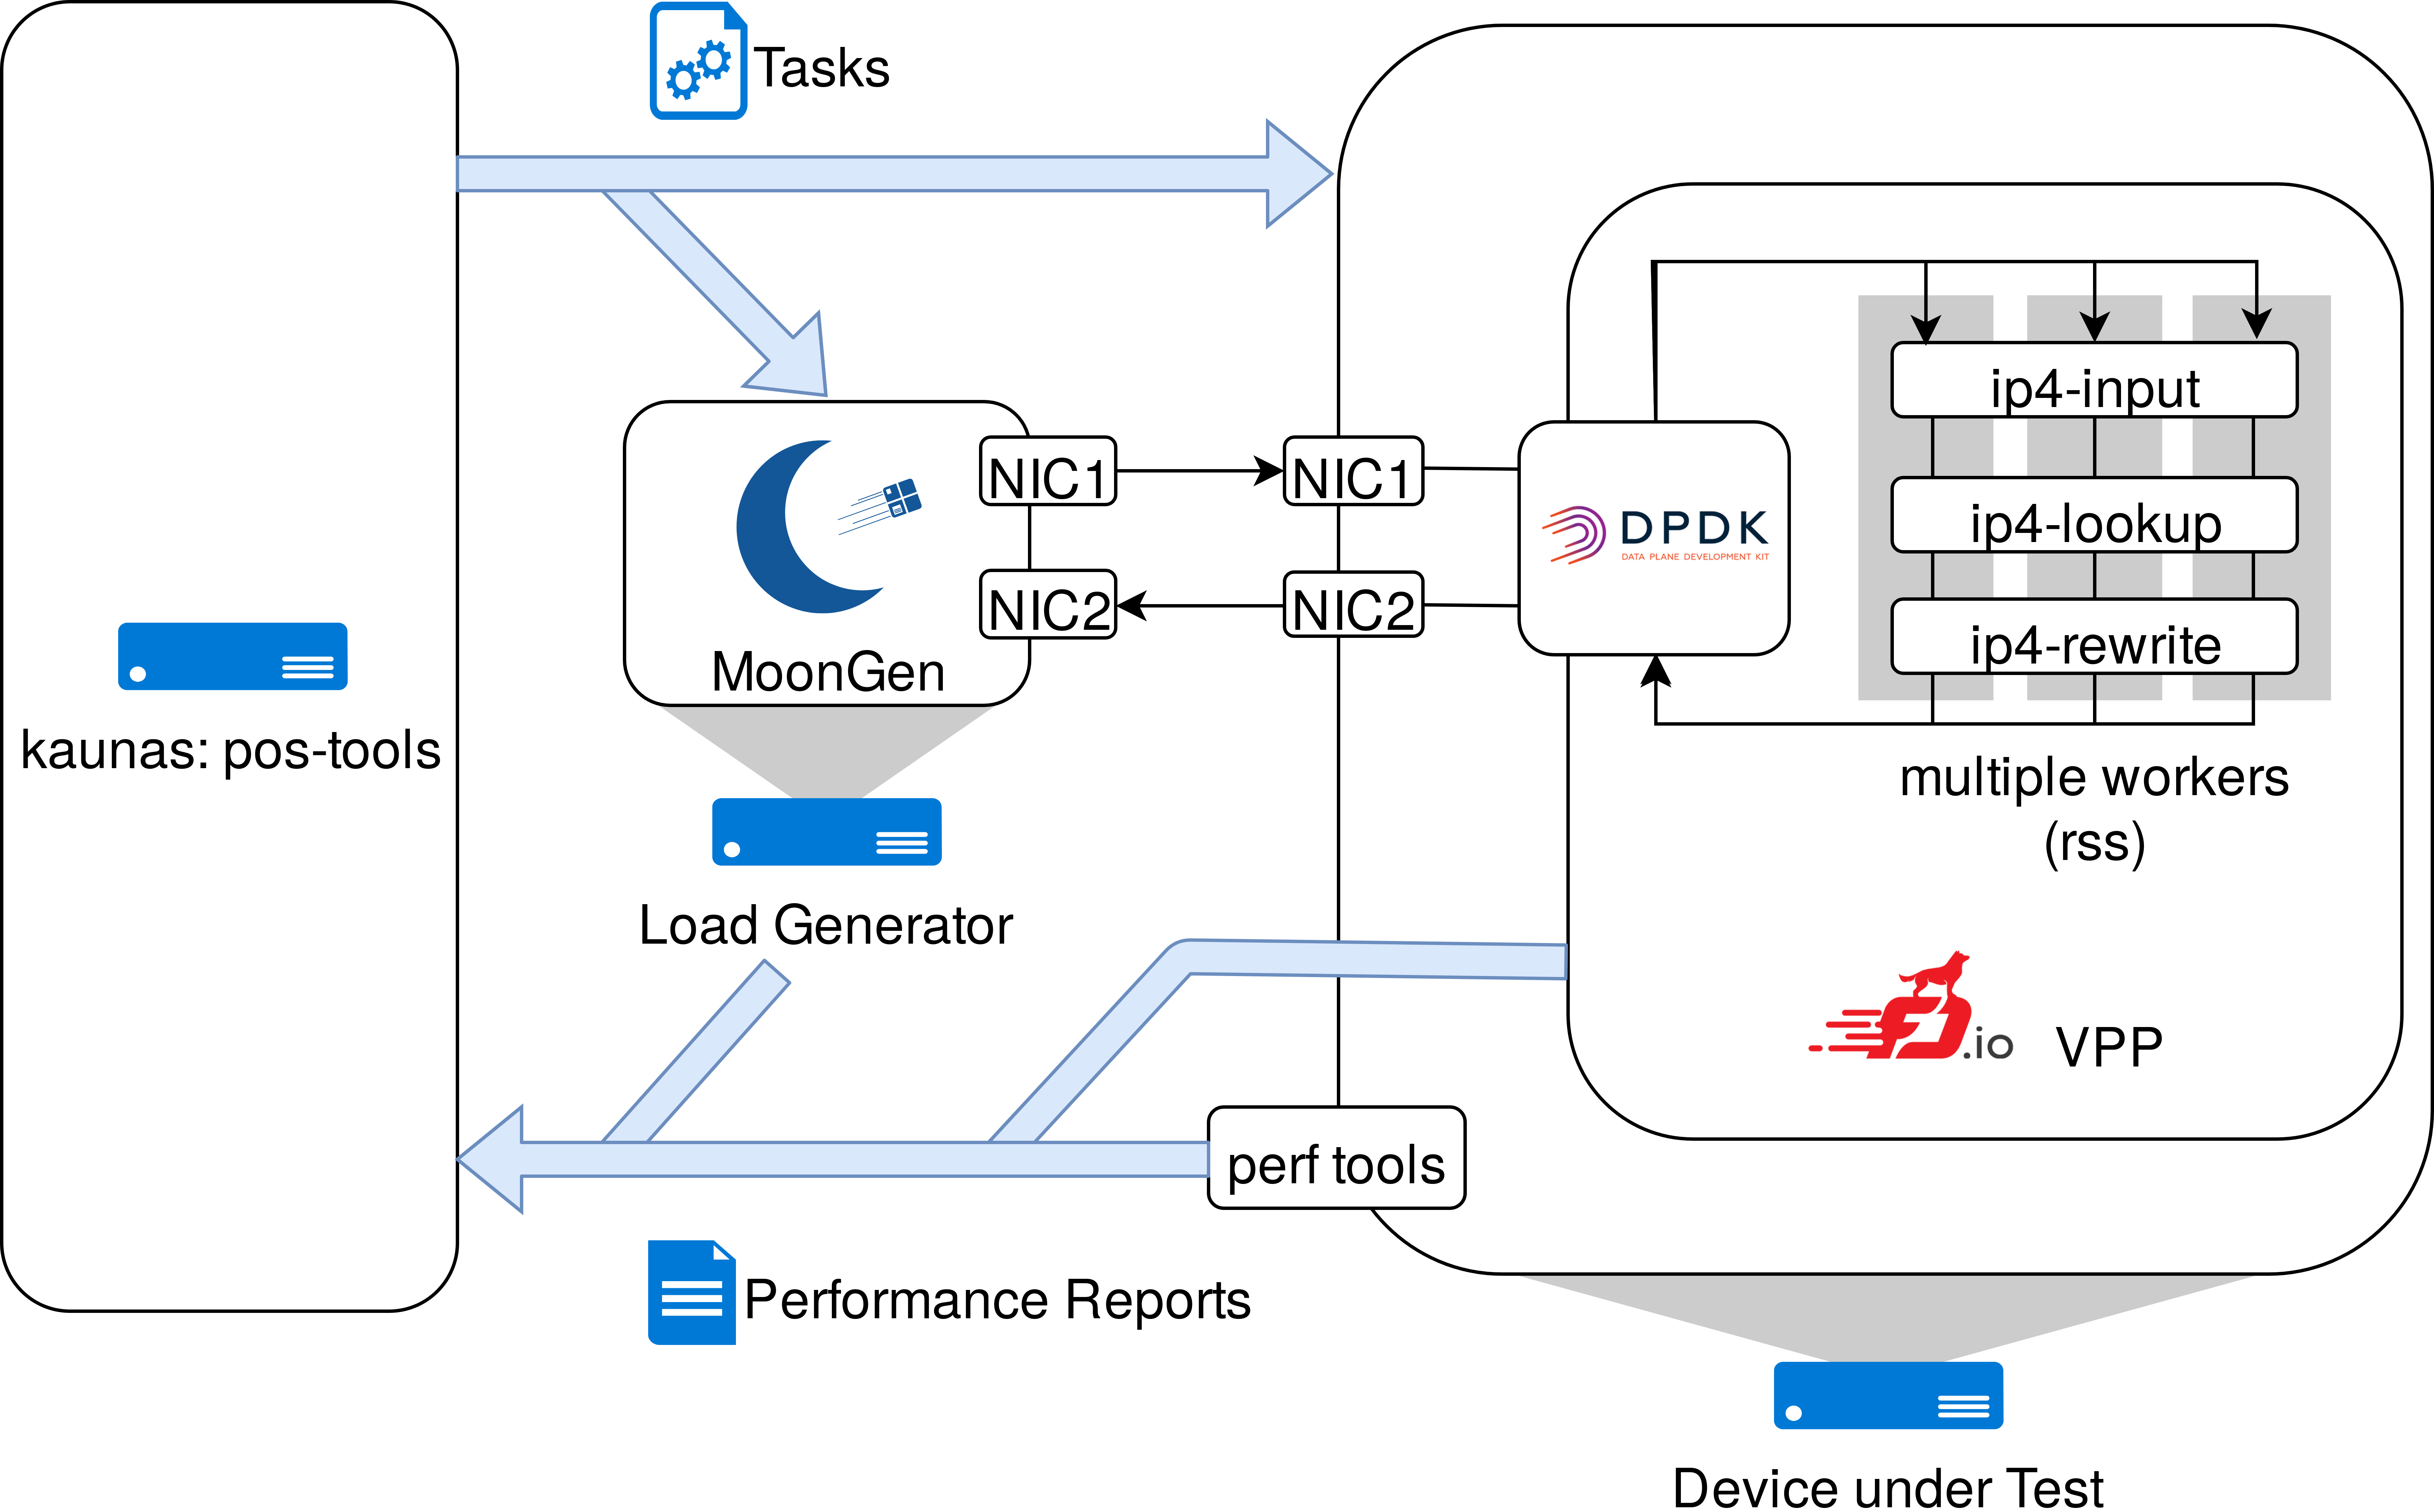
\includegraphics[width=\linewidth]{pics/topology.png}
    %\caption{Experiment setup for testing VPP with "kaunas" management server, LoadGen and DUT}
    \label{setup}
    \end{figure}
\end{frame}


\begin{frame}
    \frametitle{Packet Processing Graph}
    \begin{figure}
    \noindent\hspace{1mm}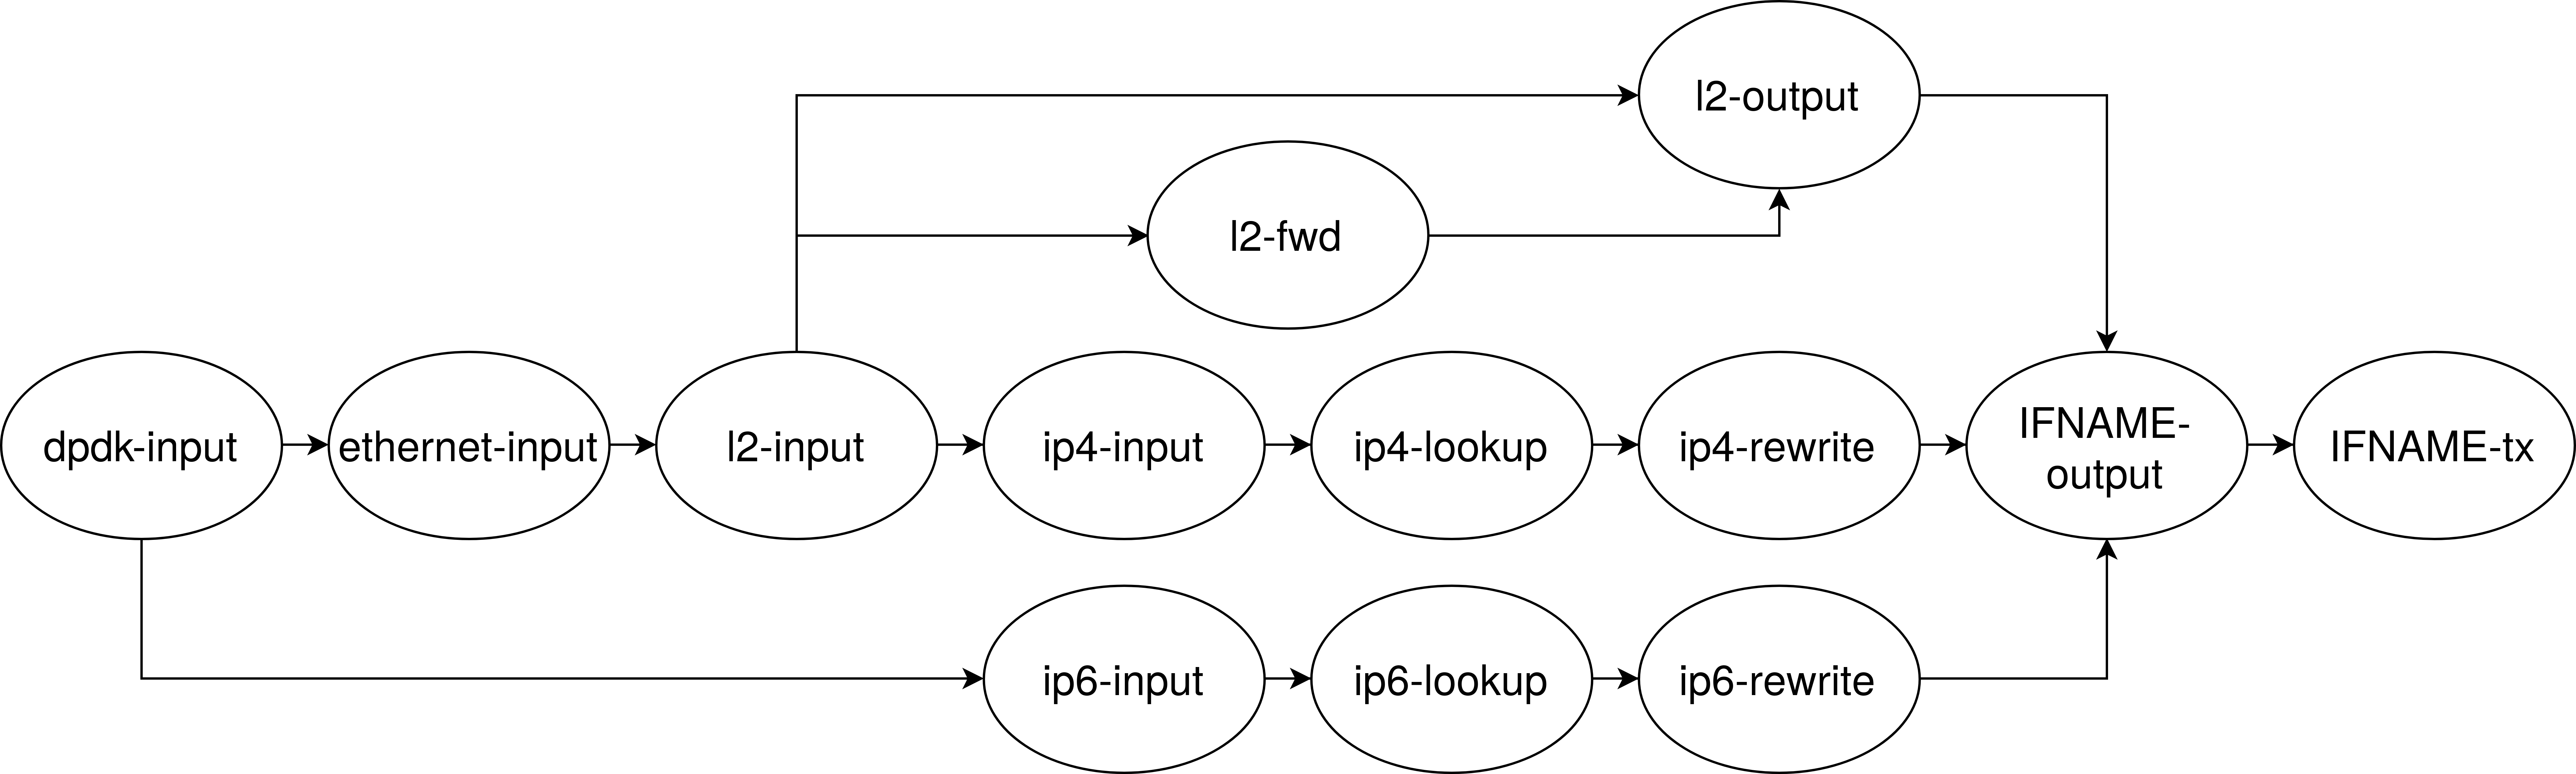
\includegraphics[width=\linewidth]{pics/vpp-nodes-horizontal.png}
    \caption{VPP packet processing graph for xconnect, bridging, IPv4 routing and IPv6 routing. Other paths are left out. }
    \label{nodegraph}
    \end{figure}
\end{frame}

\section{Tests Conducted}

\begin{frame}
    \frametitle{Scenarios}
    Scenarios:
    
\end{frame}

\begin{frame}
    \frametitle{Parameters}
\end{frame}

\section{Conclusion}


\begin{frame}
    \frametitle{Comparison}
    % TODO graphical visualization
    \begin{table}
        \begin{tabular}[]{ l r r r }
            Implementation   & FIB sizes & Mpps     & Relative \\ 
            \midrule
            MoonRoute        & 1         & 14.6     & 100\% \\
            MoonRoute        & $2^{20}$  & 14.2     & 97\% \\
            MoonRoute        & $2^{24}$  & 11.6     & 79\% \\
            VPP v18.10       & 1         & 11.6     & 79\% \\
            FastClick DPDK   & 1         & 10.4     & 72\% \\
            FastClick DPDK   & $2^{20}$  & 10.4     & 72\% \\
            VPP v16.09       & 1         & 9.7      & 71\% \\
            VPP v16.09       & 255k      & 9.2      & 63\% \\
            VPP v16.09       & $2^{20}$  & 8.5      & 58\% \\
            VPP v18.10       & 255k      & 7.2      & 50\% \\
            VPP v16.09       & $2^{23}$  & 6.5      & 45\% \\
            Click DPDK       & 1         & 4.3      & 29\% \\
            Click DPDK       & $2^{20}$  & 4.2      & 28\% \\
            Linux 3.7        & 1         & 1.5      & 11\% \\

            \midrule
        \end{tabular}
        \caption{Comparison of maximum IPv4 forwarding throughput with a single worker on the Xeon E3-1230 system. Non-VPP results are from \cite{chair:architecture} and are conducted on the same system. }
        \label{table:comparison}
    \end{table}
\end{frame}



\section{Questions?}

\begin{frame}
    \frametitle{Example frame}
    \begin{itemize}
        \item item 1
        \item $\ldots$
        \begin{itemize}
            \item test
            \item $\ldots$
        \end{itemize}
    \end{itemize}
    Citation \cite{rfc959}

    \paragraph{Math mode should be fully functional:}
    $$
    \hat s
    \overline s
    \mathcal S
    \mathbit S
    \mathbit \Lambda
    \sum
    \pd{\xi}
    \pr{X=0}
    \mathbit 1
    $$
\end{frame}

\begin{frame}
    \frametitle{Figures}
    \begin{figure}
        \centering
        \includegraphics[width=.5\textwidth]{figures/example}
        \caption{Figure caption}
        \label{Maizaso0}
    \end{figure}
    Figure~\ref{Maizaso0} shows a small network.
\end{frame}

\begin{frame}
    \frametitle{Figures}
    \begin{table}
        \begin{tabular}{rccc}
            \toprule
            & Competitor 1 & Competitor 2 & we\\
            \midrule
            Feature A & \no & \maybe & \yes\\
            Feature B & \no & \maybe & \yes\\
            Feature C & \no & \maybe & \yes\\
            Feature D & \no & \maybe & \yes\\
            \bottomrule
        \end{tabular}
    \end{table}
\end{frame}



% Include markdown source from ./pandoc
%\section{Agenda}

\begin{frame}
    \begin{itemize}
            \item item 1
            \item $\ldots$
            \begin{itemize}
                \item test
                \item $\ldots$
            \end{itemize}
        \end{itemize}
\end{frame}

\section{Next Section}

\begin{frame}
    \frametitle{Benchmarking Setup}
    \begin{figure}
    \noindent\hspace{1mm}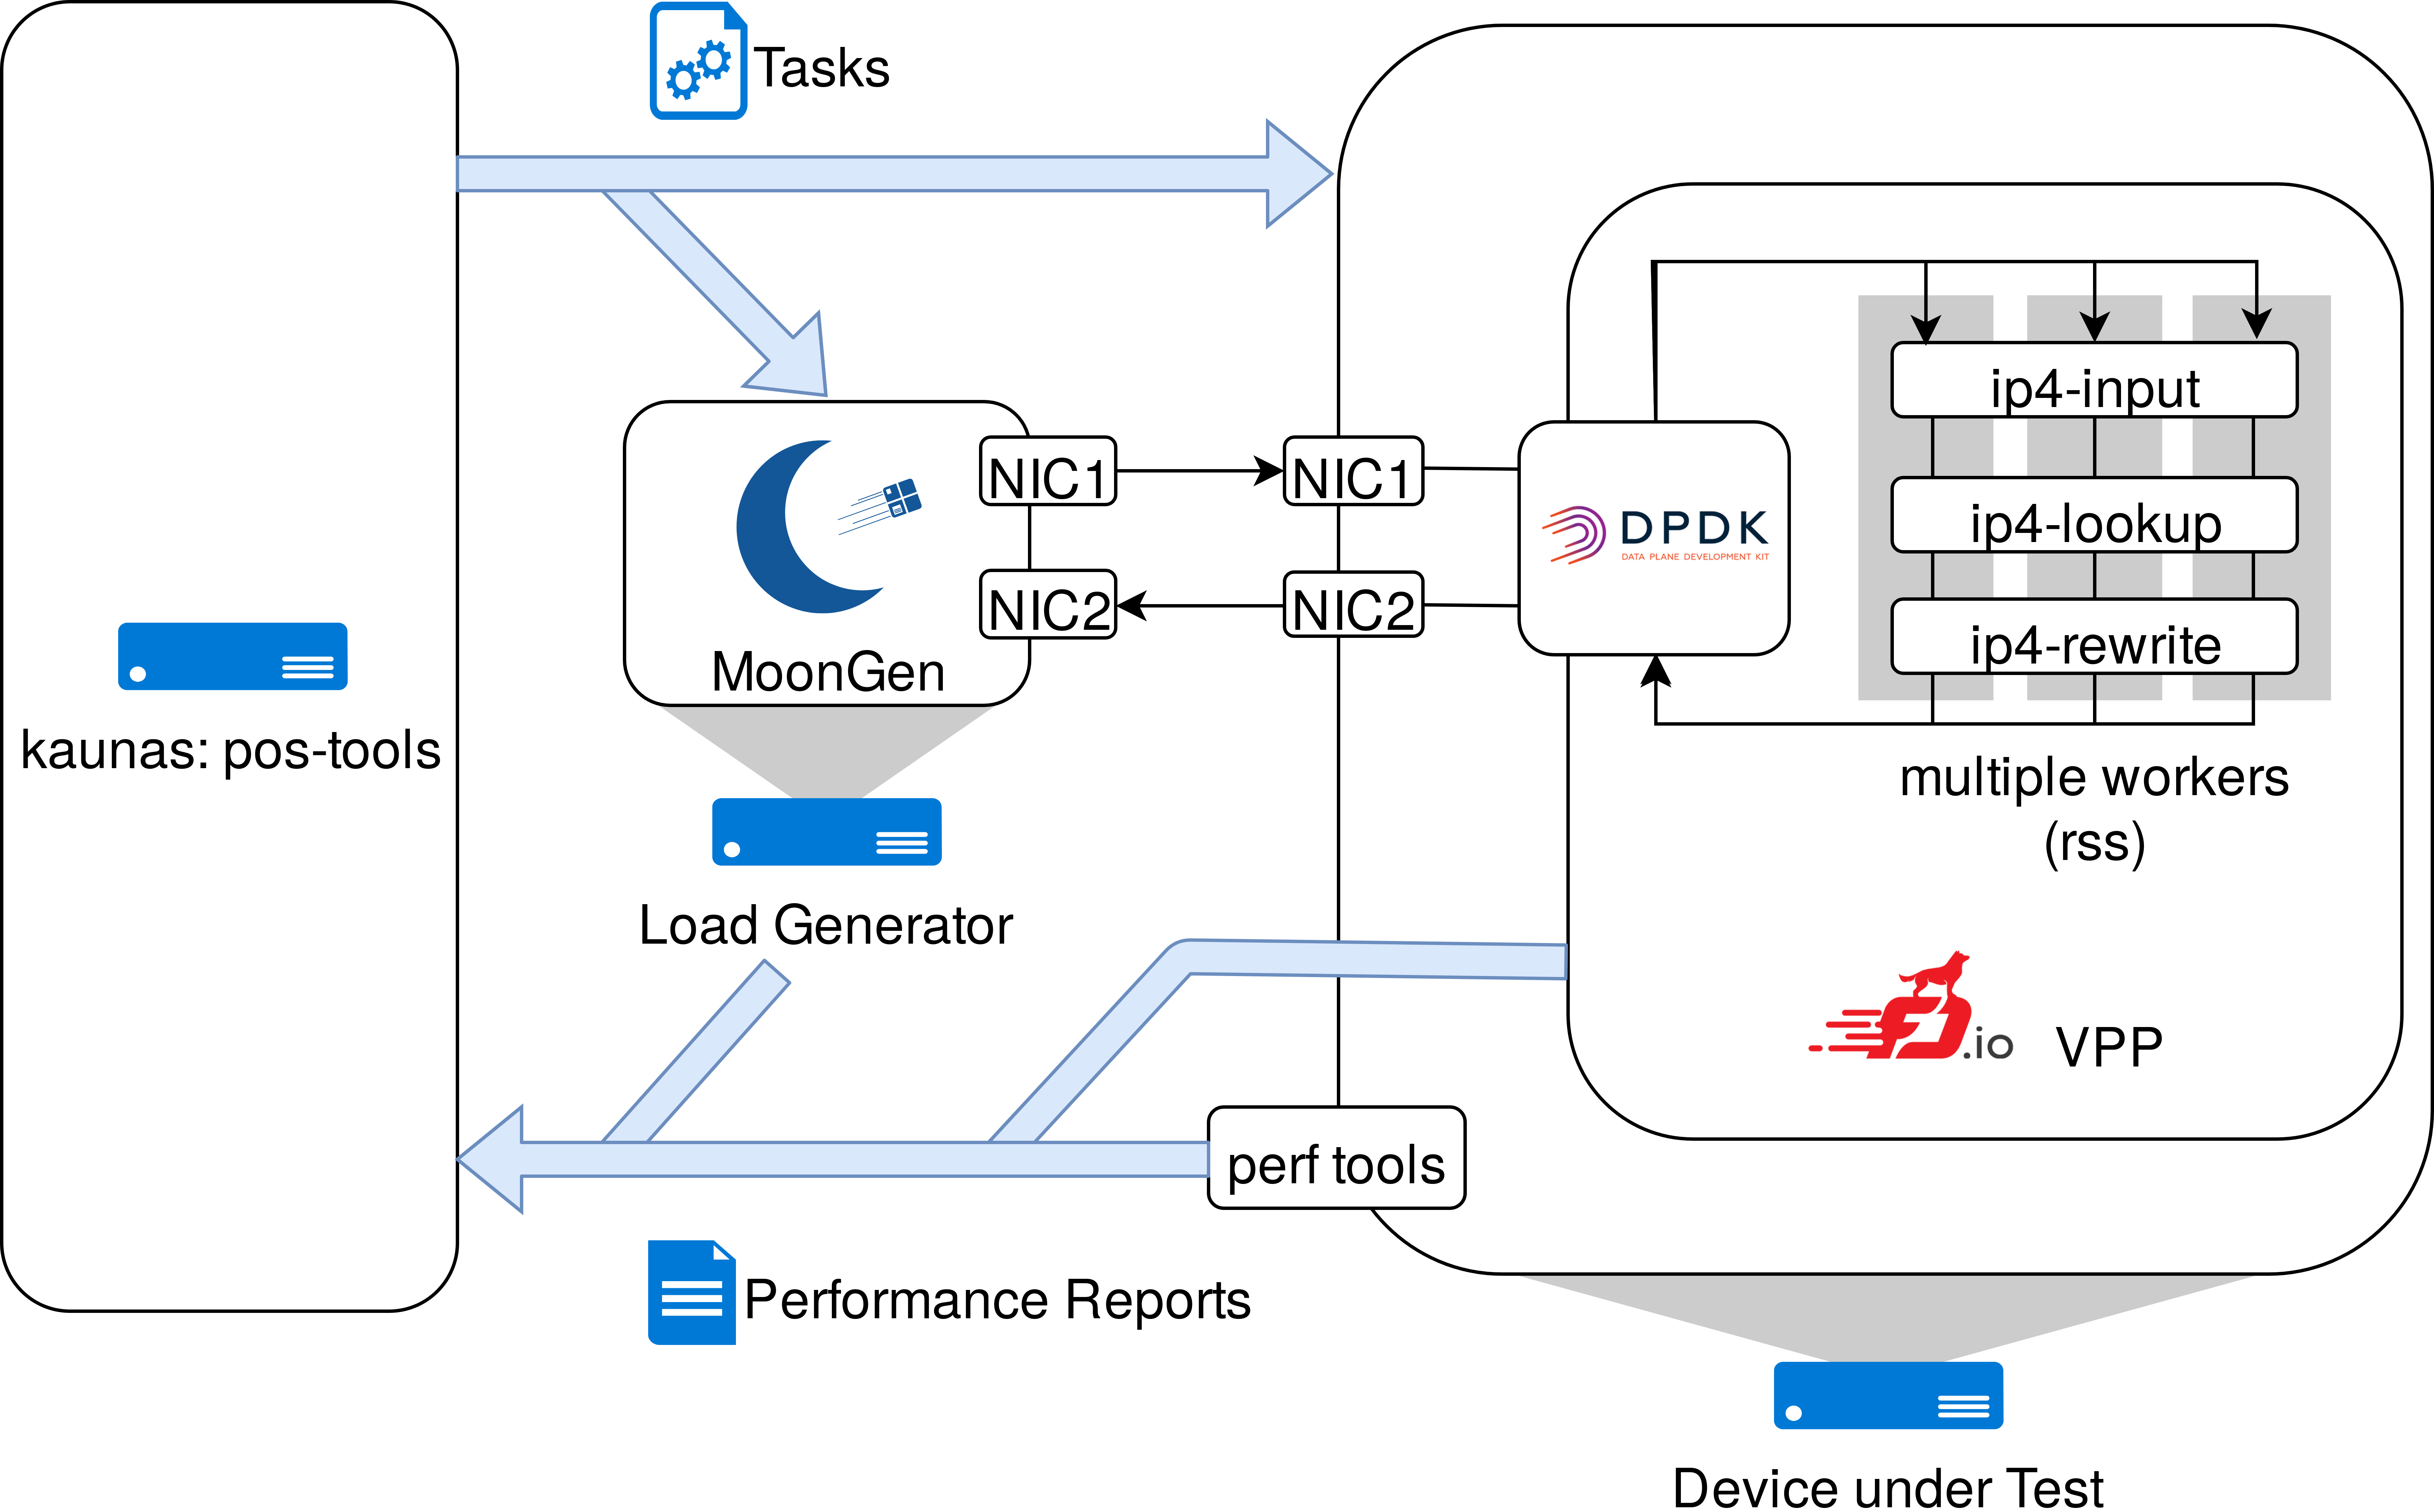
\includegraphics[width=\linewidth]{pics/topology.png}
    %\caption{Experiment setup for testing VPP with "kaunas" management server, LoadGen and DUT}
    \label{setup}
    \end{figure}
\end{frame}


\begin{frame}
    \frametitle{Packet Processing Graph}
    \begin{figure}
    \noindent\hspace{1mm}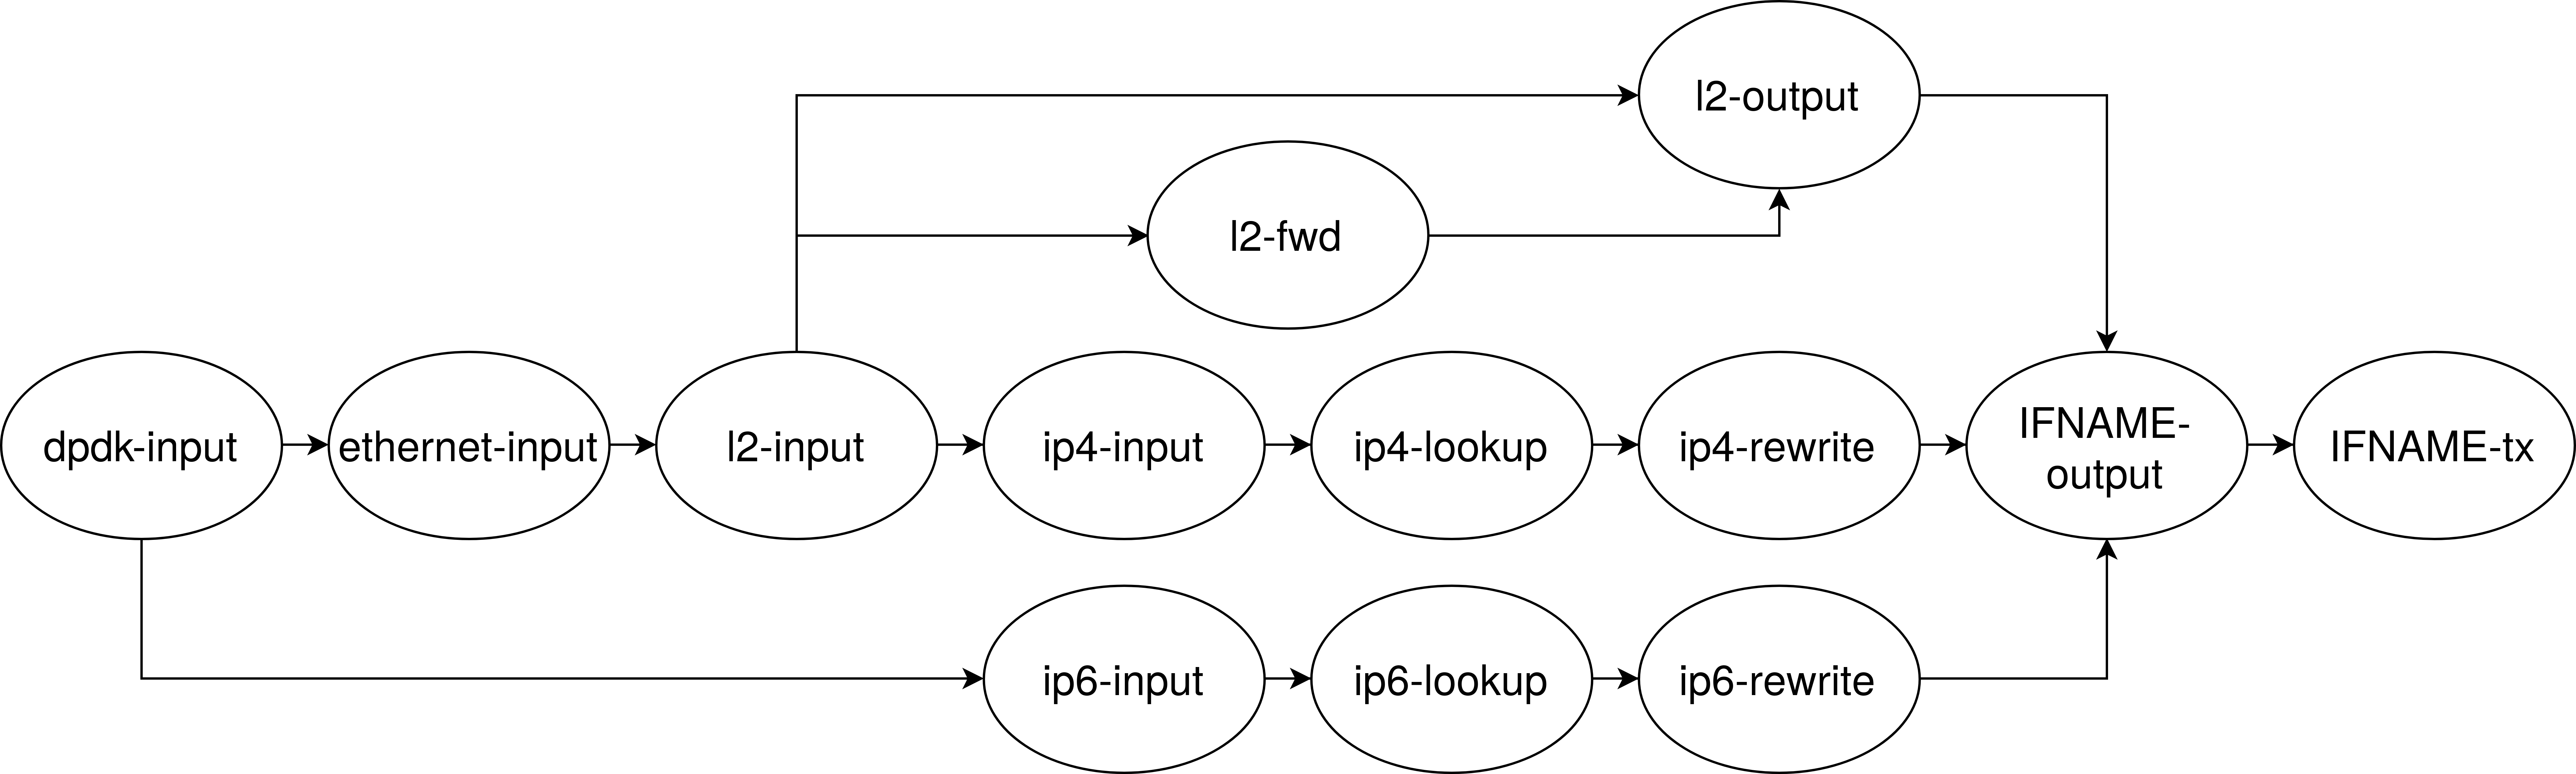
\includegraphics[width=\linewidth]{pics/vpp-nodes-horizontal.png}
    \caption{VPP packet processing graph for xconnect, bridging, IPv4 routing and IPv6 routing. Other paths are left out. }
    \label{nodegraph}
    \end{figure}
\end{frame}

\section{Tests Conducted}

\begin{frame}
    \frametitle{Scenarios}
    Scenarios:
    
\end{frame}

\begin{frame}
    \frametitle{Parameters}
\end{frame}

\section{Conclusion}


\begin{frame}
    \frametitle{Comparison}
    % TODO graphical visualization
    \begin{table}
        \begin{tabular}[]{ l r r r }
            Implementation   & FIB sizes & Mpps     & Relative \\ 
            \midrule
            MoonRoute        & 1         & 14.6     & 100\% \\
            MoonRoute        & $2^{20}$  & 14.2     & 97\% \\
            MoonRoute        & $2^{24}$  & 11.6     & 79\% \\
            VPP v18.10       & 1         & 11.6     & 79\% \\
            FastClick DPDK   & 1         & 10.4     & 72\% \\
            FastClick DPDK   & $2^{20}$  & 10.4     & 72\% \\
            VPP v16.09       & 1         & 9.7      & 71\% \\
            VPP v16.09       & 255k      & 9.2      & 63\% \\
            VPP v16.09       & $2^{20}$  & 8.5      & 58\% \\
            VPP v18.10       & 255k      & 7.2      & 50\% \\
            VPP v16.09       & $2^{23}$  & 6.5      & 45\% \\
            Click DPDK       & 1         & 4.3      & 29\% \\
            Click DPDK       & $2^{20}$  & 4.2      & 28\% \\
            Linux 3.7        & 1         & 1.5      & 11\% \\

            \midrule
        \end{tabular}
        \caption{Comparison of maximum IPv4 forwarding throughput with a single worker on the Xeon E3-1230 system. Non-VPP results are from \cite{chair:architecture} and are conducted on the same system. }
        \label{table:comparison}
    \end{table}
\end{frame}



\section{Questions?}

\begin{frame}
    \frametitle{Example frame}
    \begin{itemize}
        \item item 1
        \item $\ldots$
        \begin{itemize}
            \item test
            \item $\ldots$
        \end{itemize}
    \end{itemize}
    Citation \cite{rfc959}

    \paragraph{Math mode should be fully functional:}
    $$
    \hat s
    \overline s
    \mathcal S
    \mathbit S
    \mathbit \Lambda
    \sum
    \pd{\xi}
    \pr{X=0}
    \mathbit 1
    $$
\end{frame}

\begin{frame}
    \frametitle{Figures}
    \begin{figure}
        \centering
        \includegraphics[width=.5\textwidth]{figures/example}
        \caption{Figure caption}
        \label{Maizaso0}
    \end{figure}
    Figure~\ref{Maizaso0} shows a small network.
\end{frame}

\begin{frame}
    \frametitle{Figures}
    \begin{table}
        \begin{tabular}{rccc}
            \toprule
            & Competitor 1 & Competitor 2 & we\\
            \midrule
            Feature A & \no & \maybe & \yes\\
            Feature B & \no & \maybe & \yes\\
            Feature C & \no & \maybe & \yes\\
            Feature D & \no & \maybe & \yes\\
            \bottomrule
        \end{tabular}
    \end{table}
\end{frame}



% Comment out if you do not want a bibliography
\section{Bibliography}
\begin{frame}[allowframebreaks]
    \bibliographystyle{abbrv}
    \setbeamertemplate{bibliography item}[text]
    \footnotesize
    \bibliography{lit}
\end{frame}

\end{document}

